\documentclass[a4paper]{article}

\usepackage{hyperref}
%\hypersetup{
%colorlinks=false,              % bool: Liens colorés
%pdfborder={0 0 0}             % Ne pas encadrer les liens
%}
\usepackage[utf8]{inputenc}  
\usepackage[francais]{babel}  
\usepackage[top=2cm, bottom=2cm, left=2cm, right=2cm]{geometry}
\usepackage{graphicx}
\usepackage[final]{pdfpages} 
\usepackage{rotating}
\usepackage{eurosym}
\usepackage{lscape}
\usepackage{float}
% définir les commandes ici

% s'il y a beaucoup de commandes et de packages à inclure n'h&ésitez pas
% à mettre tout ça dans un fichier include.tex et l'inclure
% \input{include.tex}


\begin{document}

%------------------------------------- Page de titre
\begin{titlepage}
~ 
\vfill
	\begin{center}
		\begin{Huge}
		SOA : Dossier d'Architecture Technique\\
		\end{Huge} 
\vfill
		\textbf{Hexanome 4211 :} 
		\\Sandra \bsc{Mondain}, Elisa \bsc{Abidh}, 
		\\Gaël \bsc{Motte}, Armand \bsc{Rossius}, 
		\\Rémi \bsc{Fradet}, Nicolas \bsc{Silva}, Julien \bsc{Levesy}\\

\vfill		
		\begin{Large}
		Avril 2011
		\end{Large}
\vfill
	\begin{tabular}{|c|c|c|c|c|}
 	 \hline
 	 Auteur du Document & Responsable Validation & Phase & Etat & Avancement \\
 	 \hline
 	 
 	\hline
 	
	\end{tabular}
\vfill	
	\end{center}
\vfill
\end{titlepage}
%----------------------------------------------------

%--------------------------------- Table des matières
\newpage
\tableofcontents
\newpage
%----------------------------------------------- Plan

\section{TODO titre section}

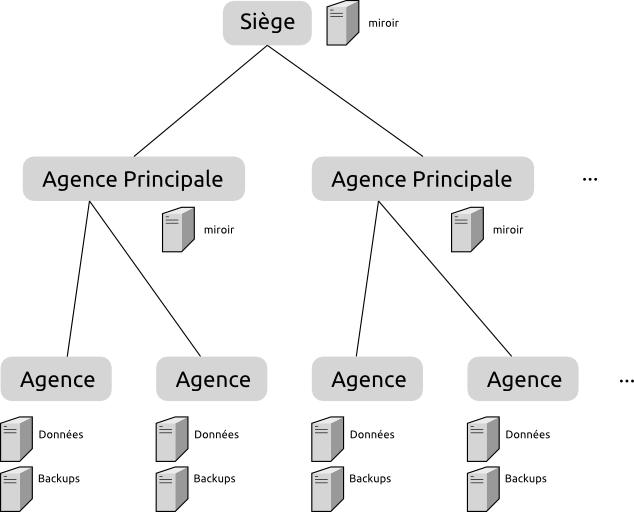
\includegraphics{archi_base.png}

Un tel système nécessite une architecture à la fois distribuée et synchronisée.
au sein de chaque agence les données sont centralisées rsur un serveur (et répliquées sur un ou plusieurs serveur d'archivage pour des raisons de sécurité).\\
Les serveurs de chaque agence sont situés dans les réseaux internes des agences et forment un réseau et communiquent par VPN aux serveur miroir de l'agence principale de leur région. 
Ces serveurs \textit{miroirs} dupliquent les données des agences affiliées à l'agence principale et mettent à jour informations régulièrement et sur demande.
Les serveurs miroirs des agences principales permettent d'avoir une vue sur l'activité de l'entreprise au niveau régionnal.\\
Le même processus de réplication hierarchisé s'applique au niveau supérieur, c'est à dire au niveau du Siège de l'entreprise, qui possède des serveurs miroirs dupliquant des données provenant de toutes les agences.\\
Afin de limiter le volume de donner à transferer et à stocker, les miroirs appliquent des filtres sur les données afin de ne conserver que des informations utiles, comme par exemple ne pas conserver dans les miroirs les agendas de dates considérées anciennes. Ces miroirs ont pour but d'alléger la charge réseau liée au transfert de données entre agence ainsi que conserver une certaine visibilité sur l'activité même en cas de dysfonctionnement quelque part sur le réseau, et non d'archiver les données.


\end{document}
